\documentclass[aspectratio=169,xcolor=table]{beamer}

\usepackage{basileabeam}
\usepackage[english]{babel}
\usepackage[T1]{fontenc}
\usepackage{xcolor}
\usepackage{amssymb}
\usepackage{mathtools}
\usepackage{booktabs}
\usepackage{graphicx}
\usepackage{listings}
\usepackage{tikz}
\usetikzlibrary{arrows.meta,backgrounds,calc,fit,positioning,shapes.geometric}

\definecolor{unimint}{RGB}{30,165,165}
\definecolor{unilightmint}{RGB}{165,215,210}
\definecolor{unidark}{RGB}{45,55,60}
\definecolor{unigrey}{RGB}{140,145,150}
\definecolor{unired}{RGB}{210,5,55}
\definecolor{softblue}{RGB}{232,242,250}
\definecolor{softmint}{RGB}{232,247,245}
\definecolor{softred}{RGB}{252,235,239}
\definecolor{softgrey}{RGB}{244,245,246}

\setbeamerfont{footnote}{size=\tiny}
\setbeamerfont{caption}{size=\scriptsize}
\setbeamertemplate{caption}[numbered]
\setbeamercovered{invisible}

\newcommand{\code}[1]{\texttt{#1}}
\newcommand{\key}[1]{\textcolor{unired}{\textbf{#1}}}
\newcommand{\implemented}{\textcolor{unimint}{\textbf{Implemented}}}
\newcommand{\planned}{\textcolor{unired}{\textbf{Planned}}}

\tikzset{
  >={Latex[length=2.2mm]},
  flow/.style={-Latex, line width=0.75pt, draw=unidark},
  flowsoft/.style={-Latex, line width=0.65pt, draw=unigrey},
  box/.style={
    draw=unidark,
    rounded corners=1.5pt,
    fill=white,
    align=center,
    inner sep=4.5pt,
    font=\scriptsize
  },
  mintbox/.style={box, fill=softmint, draw=unimint},
  bluebox/.style={box, fill=softblue, draw=blue!55!black},
  redbox/.style={box, fill=softred, draw=unired},
  greybox/.style={box, fill=softgrey, draw=unigrey},
  groupbox/.style={
    draw=unigrey,
    rounded corners=2pt,
    fill=softgrey,
    inner sep=7pt
  },
  tinylabel/.style={font=\tiny, text=unigrey, align=center}
}

\lstset{
  basicstyle=\ttfamily\tiny,
  keywordstyle=\color{unired}\bfseries,
  commentstyle=\color{unigrey},
  stringstyle=\color{blue!60!black},
  showstringspaces=false,
  columns=fullflexible,
  keepspaces=true,
  frame=single,
  rulecolor=\color{unigrey},
  backgroundcolor=\color{softgrey},
  xleftmargin=0.25em,
  xrightmargin=0.25em,
  aboveskip=0.3em,
  belowskip=0.3em
}


\title{Bachelor Thesis Midterm}
\subtitle{A Multimodal XR Museum with vitrivr and Godot}
\author{Jannick Seper}
\institute{University of Basel}
\date{22 July 2026}

\ulogo{Template/header}
\ulistelement{Template/listelement}
\graphicspath{{./images/}{../}}
\totalNoSlidesDisabled

\begin{document}

% Slide 01: Bachelor Thesis Midterm
\begin{frame}[t,plain]
  \titlepage
\end{frame}

\input{content/02-key-terms}
% Slide 03: Starting point
\section{Motivation}
\begin{frame}[c]{Starting point}
\begin{columns}[T,onlytextwidth]
  \begin{column}{0.44\textwidth}
    \textcolor{unigrey}{\large PREDECESSOR}

    \vspace{0.12cm}
    \Large VIRTUE

    \vspace{0.15cm}
    \small
    \begin{itemize}
      \item dynamically arranged image galleries in VR
      \item retrieval with spatial exploration
      \item Cineast and Cottontail DB
      \item image collections
    \end{itemize}
  \end{column}
  \begin{column}{0.08\textwidth}
    \vspace{1.45cm}
    \centering
    \Huge$\rightarrow$
  \end{column}
  \begin{column}{0.44\textwidth}
    \textcolor{unimint}{\large THIS THESIS}

    \vspace{0.12cm}
    \Large Multimodal XR museum

    \vspace{0.15cm}
    \small
    \begin{itemize}
      \item vitrivr-engine and pgvector
      \item images, videos, and 3D models
      \item multiple headsets through OpenXR
      \item similarity as an interaction
    \end{itemize}
  \end{column}
\end{columns}
\end{frame}

% Slide 04: Three project goals
\begin{frame}[c]{Three project goals}
\begin{columns}[T,onlytextwidth]
  \begin{column}{0.31\textwidth}
    \textcolor{unired}{\LARGE 01}

    \vspace{0.1cm}
    \large \textbf{Retrieve}

    \vspace{0.12cm}
    \color{unimint}\rule{\linewidth}{1.6pt}

    \vspace{0.2cm}
    \small
    vitrivr-engine and pgvector provide semantic search over multimodal embeddings.
  \end{column}
  \begin{column}{0.31\textwidth}
    \textcolor{unired}{\LARGE 02}

    \vspace{0.1cm}
    \large \textbf{Experience}

    \vspace{0.12cm}
    \color{unimint}\rule{\linewidth}{1.6pt}

    \vspace{0.2cm}
    \small
    The XR application presents retrieved images, videos, and 3D models as interactive exhibits.
  \end{column}
  \begin{column}{0.31\textwidth}
    \textcolor{unired}{\LARGE 03}

    \vspace{0.1cm}
    \large \textbf{Explore}

    \vspace{0.12cm}
    \color{unimint}\rule{\linewidth}{1.6pt}

    \vspace{0.2cm}
    \small
    Users trigger new similarity searches from exhibits.
  \end{column}
\end{columns}
\end{frame}

% Slide 05: System overview
\section{System}
\begin{frame}[c]{System overview}
\begin{columns}[T,onlytextwidth]
  \begin{column}{0.31\textwidth}
    \textcolor{unired}{\LARGE 01}

    \vspace{0.1cm}
    \large\textbf{VR application}

    \vspace{0.12cm}
    \color{unimint}\rule{\linewidth}{1.6pt}
    \color{black}

    \raggedright
    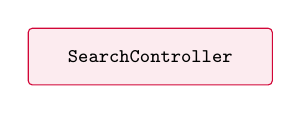
\begin{tikzpicture}[remember picture]
      \node[redbox,minimum width=3.10cm,minimum height=0.72cm]
        (search) {\code{SearchController}};
    \end{tikzpicture}

    \vspace{0.28cm}
    \raggedright\small
    \textbf{Input and interaction}\\
    keyboard, controllers, hand tracking

    \vspace{0.34cm}
    \textbf{Placement strategies}\\
    wall slots, 3D stands
  \end{column}

  \begin{column}{0.31\textwidth}
    \textcolor{unired}{\LARGE 02}

    \vspace{0.1cm}
    \large\textbf{.NET application}

    \vspace{0.12cm}
    \color{unimint}\rule{\linewidth}{1.6pt}
    \color{black}

    \raggedright
    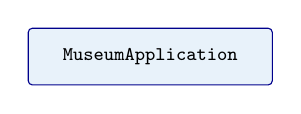
\begin{tikzpicture}[remember picture]
      \node[bluebox,minimum width=3.10cm,minimum height=0.72cm]
        (application) {\code{MuseumApplication}};
    \end{tikzpicture}

    \vspace{0.28cm}
    \raggedright\small
    \textbf{Use cases}\\
    search, validation

    \vspace{0.34cm}
    \textbf{Adapters}\\
    request, parser, loader
  \end{column}

  \begin{column}{0.31\textwidth}
    \textcolor{unired}{\LARGE 03}

    \vspace{0.1cm}
    \large\textbf{Retrieval + delivery}

    \vspace{0.12cm}
    \color{unimint}\rule{\linewidth}{1.6pt}
    \color{black}

    \raggedright
    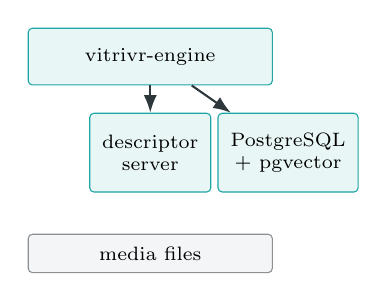
\begin{tikzpicture}[remember picture]
      \node[mintbox,minimum width=3.10cm,minimum height=0.72cm]
        (engine) at (0,0) {vitrivr-engine};
      \node[mintbox,minimum width=1.50cm,minimum height=1cm]
        (descriptor) at (0,-1.22) {descriptor\\server};
      \node[mintbox,minimum width=1.50cm,minimum height=1cm]
        (database) at (1.75,-1.22) {PostgreSQL\\+ pgvector};
      \node[greybox,minimum width=3.10cm]
        (files) at (0,-2.5) {media files};

      \draw[flow] (engine) -- (descriptor);
      \draw[flow] (engine) -- (database);
    \end{tikzpicture}
  \end{column}
\end{columns}

\begin{tikzpicture}[remember picture,overlay]
  \draw[flow] (search.east) -- node[above=2pt,tinylabel] {text or vector} (application.west);
  \draw[flow] (application.east) -- node[above=2pt,tinylabel] {REST query} (engine.west);
  \draw[flowsoft] (application.south east) to[out=-1,in=160]
    node[above=2pt, right ,tinylabel] {local path\\or HTTP} (files.west);
\end{tikzpicture}
\end{frame}

\input{content/06-clip-retrieval}
% Slide 07: 3D retrieval
\begin{frame}[c]{3D retrieval}
\centering
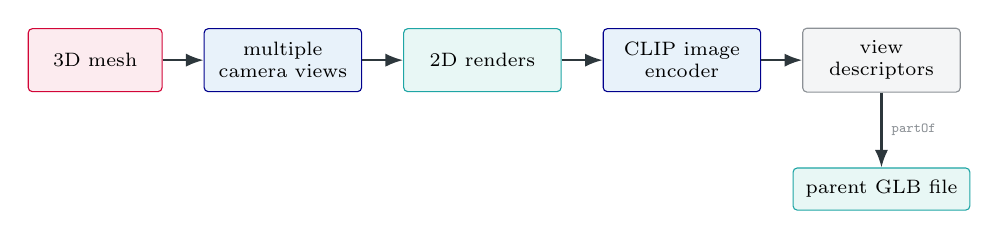
\begin{tikzpicture}[node distance=0.52cm, every node/.style={font=\scriptsize}]
  \node[redbox, minimum width=1.7cm, minimum height=0.8cm] (mesh) {3D mesh};
  \node[bluebox, right=of mesh, minimum width=2.0cm, minimum height=0.8cm] (views) {multiple\\camera views};
  \node[mintbox, right=of views, minimum width=2.0cm, minimum height=0.8cm] (renders) {2D renders};
  \node[bluebox, right=of renders, minimum width=2.0cm, minimum height=0.8cm] (clip) {CLIP image\\encoder};
  \node[greybox, right=of clip, minimum width=2.0cm, minimum height=0.8cm] (vectors) {view\\descriptors};

  \draw[flow] (mesh) -- (views);
  \draw[flow] (views) -- (renders);
  \draw[flow] (renders) -- (clip);
  \draw[flow] (clip) -- (vectors);

  \node[mintbox, below=0.95cm of vectors, minimum width=2.0cm] (parent) {parent GLB file};
  \draw[flow] (vectors) -- node[right,tinylabel] {\code{partOf}} (parent);

\end{tikzpicture}

\vspace{0.45cm}
\begin{beamercolorbox}[sep=0.5em,rounded=true]{palette highlight}
\small
Rather than encoding the mesh itself, the system searches over rendered views.
A matching view is linked through \code{partOf} to the original GLB model,
which is then loaded into the museum.
\end{beamercolorbox}
\end{frame}

\input{content/08-vitrivr-request}
% Slide 09: Godot and vitrivr remain replaceable
\section{Implementation}
\begin{frame}[c]{Godot and vitrivr remain replaceable}
\centering
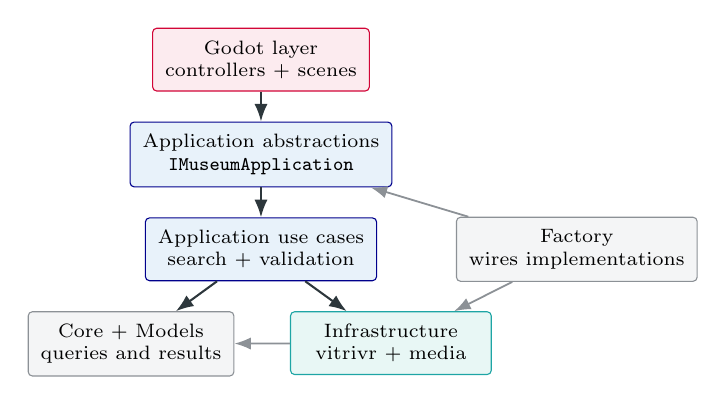
\begin{tikzpicture}[node distance=0.38cm and 0.55cm, every node/.style={font=\scriptsize}]
  \node[redbox, minimum width=2.7cm] (godot)
    {Godot layer\\controllers + scenes};
  \node[bluebox, below=of godot, minimum width=2.7cm] (abstractions)
    {Application abstractions\\\code{IMuseumApplication}};
  \node[bluebox, below=of abstractions, minimum width=2.7cm] (application)
    {Application use cases\\search + validation};
  \node[greybox, below=of application, xshift=-1.65cm, minimum width=2.55cm] (core)
    {Core + Models\\queries and results};
  \node[mintbox, below=of application, xshift=1.65cm, minimum width=2.55cm] (infra)
    {Infrastructure\\vitrivr + media};

  \draw[flow] (godot) -- (abstractions);
  \draw[flow] (abstractions) -- (application);
  \draw[flow] (application) -- (core);
  \draw[flow] (application) -- (infra);
  \draw[flowsoft] (infra) -- (core);

  \node[greybox, right=1.0cm of application, minimum width=2.3cm] (factory)
    {Factory\\wires implementations};
  \draw[flowsoft] (factory) -- (abstractions);
  \draw[flowsoft] (factory) -- (infra);
\end{tikzpicture}

\end{frame}

\input{content/10-why-godot}
\input{content/11-godot-scene-tree}
\input{content/12-entering-the-museum}
% Slide 13: Media become exhibits
\begin{frame}[c]{Media become exhibits}
\centering
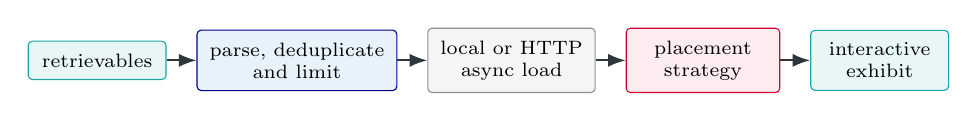
\begin{tikzpicture}[node distance=0.38cm,every node/.style={font=\scriptsize}]
  \node[mintbox,minimum width=1.75cm] (response) {retrievables};
  \node[bluebox,right=of response,minimum width=1.95cm] (prepare) {parse, deduplicate\\and limit};
  \node[greybox,right=of prepare,minimum width=1.80cm] (load) {local or HTTP\\async load};
  \node[redbox,right=of load,minimum width=1.95cm] (place) {placement\\strategy};
  \node[mintbox,right=of place,minimum width=1.75cm] (exhibit) {interactive\\exhibit};

  \foreach \a/\b in {response/prepare,prepare/load,load/place,place/exhibit}
    \draw[flow] (\a) -- (\b);
\end{tikzpicture}

\vspace{0.50cm}
\begin{columns}[T,onlytextwidth]
  \begin{column}{0.46\textwidth}
    \textcolor{unired}{\large\textbf{2D MEDIA}}

    \vspace{0.10cm}
    \color{unimint}\rule{\linewidth}{1.6pt}
    \color{black}

    \vspace{0.14cm}
    \small
    Images and videos use centred wall slots and aspect-aware frames.
  \end{column}
  \begin{column}{0.46\textwidth}
    \textcolor{unired}{\large\textbf{3D MODELS}}

    \vspace{0.10cm}
    \color{unimint}\rule{\linewidth}{1.6pt}
    \color{black}

    \vspace{0.14cm}
    \small
    GLB objects are instanced on stands and fitted to their bounds.
  \end{column}
\end{columns}

\vspace{0.42cm}
\begin{beamercolorbox}[sep=0.55em,rounded=true]{palette highlight}
  \centering\small
  Every exhibit stores its path, name, and CLIP vector for \textbf{Similar}.
  3D models also support \textbf{Original Size}.
\end{beamercolorbox}

\end{frame}

\input{content/14-current-status}
% Slide 15: Demo
\section{Demo}
\begin{frame}[c,plain]
\centering
\Huge Demo

\vspace{0.65cm}
\large
Search $\rightarrow$ explore $\rightarrow$ inspect $\rightarrow$ search again

\end{frame}

% Slide 16: Evaluation questionnaire
\section{Evaluation}
\begin{frame}[c]{Evaluation questionnaire}
\begin{columns}[T,onlytextwidth]
  \begin{column}{0.31\textwidth}
    \textcolor{unired}{\LARGE 01}

    \vspace{0.08cm}
    \parbox[t][0.82cm][t]{\linewidth}{\large\bfseries SUS}

    \vspace{0.04cm}
    \color{unimint}\rule{\linewidth}{1.6pt}
    \color{black}

    \vspace{0.24cm}
    \large
    10 standard statements about usability.
  \end{column}

  \begin{column}{0.31\textwidth}
    \textcolor{unired}{\LARGE 02}

    \vspace{0.08cm}
    \parbox[t][0.82cm][t]{\linewidth}{\large\bfseries Project questions}

    \vspace{0.04cm}
    \color{unimint}\rule{\linewidth}{1.6pt}
    \color{black}

    \vspace{0.24cm}
    \large
    Navigation, controls, responsiveness, 3D interaction, and design.
  \end{column}

  \begin{column}{0.31\textwidth}
    \textcolor{unired}{\LARGE 03}

    \vspace{0.08cm}
    \parbox[t][0.82cm][t]{\linewidth}{\large\bfseries Context + feedback}

    \vspace{0.04cm}
    \color{unimint}\rule{\linewidth}{1.6pt}
    \color{black}

    \vspace{0.24cm}
    \large
    VR experience, device, usage mode, and one open question.
  \end{column}
\end{columns}

\end{frame}

% Slide 17: Next steps
\section{Outlook}
\begin{frame}[c]{Next steps}
\begin{columns}[T,onlytextwidth]
  \begin{column}{0.55\textwidth}
    \small
    \begin{enumerate}
      \item Reduce 3D asset sizes and resolve unsupported-material issues.
      \item Integrate and test streaming to Apple Vision Pro.
      \item Run user evaluations.
      \item Complete the reproducible setup and documentation.
      \item Finish the thesis.
    \end{enumerate}
  \end{column}
  \begin{column}{0.40\textwidth}
    \textcolor{unired}{\large\textbf{TAKEAWAY}}

    \vspace{0.12cm}
    \color{unimint}\rule{\linewidth}{1.6pt}

    \vspace{0.22cm}
    \small
    The prototype modernises the VIRTUE stack and already closes the loop from semantic query to spatial exploration.

    \vspace{0.35cm}
    Godot turns retrieval results into a device-aware XR experience.
  \end{column}
\end{columns}

\end{frame}


\end{document}
